% (The MIT License)
%
% Copyright (c) 2023-2024 Yegor Bugayenko
%
% Permission is hereby granted, free of charge, to any person obtaining a copy
% of this software and associated documentation files (the 'Software'), to deal
% in the Software without restriction, including without limitation the rights
% to use, copy, modify, merge, publish, distribute, sublicense, and/or sell
% copies of the Software, and to permit persons to whom the Software is
% furnished to do so, subject to the following conditions:
%
% The above copyright notice and this permission notice shall be included in all
% copies or substantial portions of the Software.
%
% THE SOFTWARE IS PROVIDED 'AS IS', WITHOUT WARRANTY OF ANY KIND, EXPRESS OR
% IMPLIED, INCLUDING BUT NOT LIMITED TO THE WARRANTIES OF MERCHANTABILITY,
% FITNESS FOR A PARTICULAR PURPOSE AND NONINFRINGEMENT. IN NO EVENT SHALL THE
% AUTHORS OR COPYRIGHT HOLDERS BE LIABLE FOR ANY CLAIM, DAMAGES OR OTHER
% LIABILITY, WHETHER IN AN ACTION OF CONTRACT, TORT OR OTHERWISE, ARISING FROM,
% OUT OF OR IN CONNECTION WITH THE SOFTWARE OR THE USE OR OTHER DEALINGS IN THE
% SOFTWARE.

\documentclass{article}
\usepackage{../lecture-notes.sty/lecture-notes}
\newcommand*\thetitle{Defects Density}
\begin{document}

\plush{\lnTitlePage{18}{24}{}}

\lnQuote
  [Michael Fagan]
  {michael-fagan}
  {Feedback of results from inspections must be counted for the programmer's use and \ul{benefit}: they \ul{should not} under any circumstances be used for programmer performance \ul{appraisal}.}
  {fagan1976design}

\lnPitch{
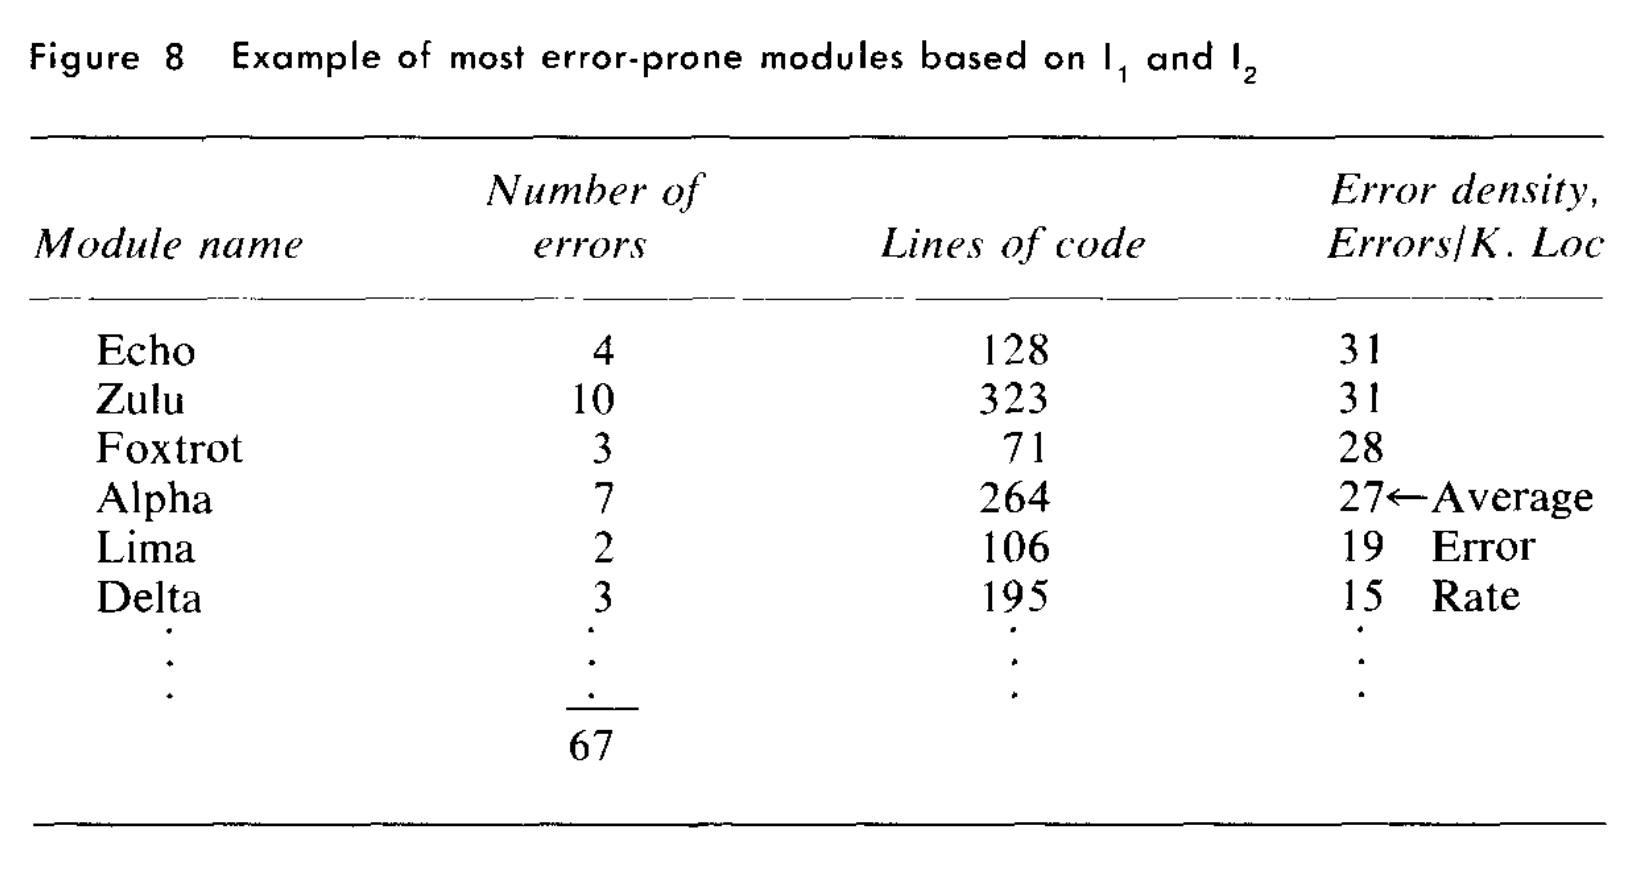
\includegraphics[width=.8\linewidth]{error-density.png}
\par
{\scriptsize Source: \bibentry{fagan1976design}\par}}

\lnPitch{\begin{multicols}{2}
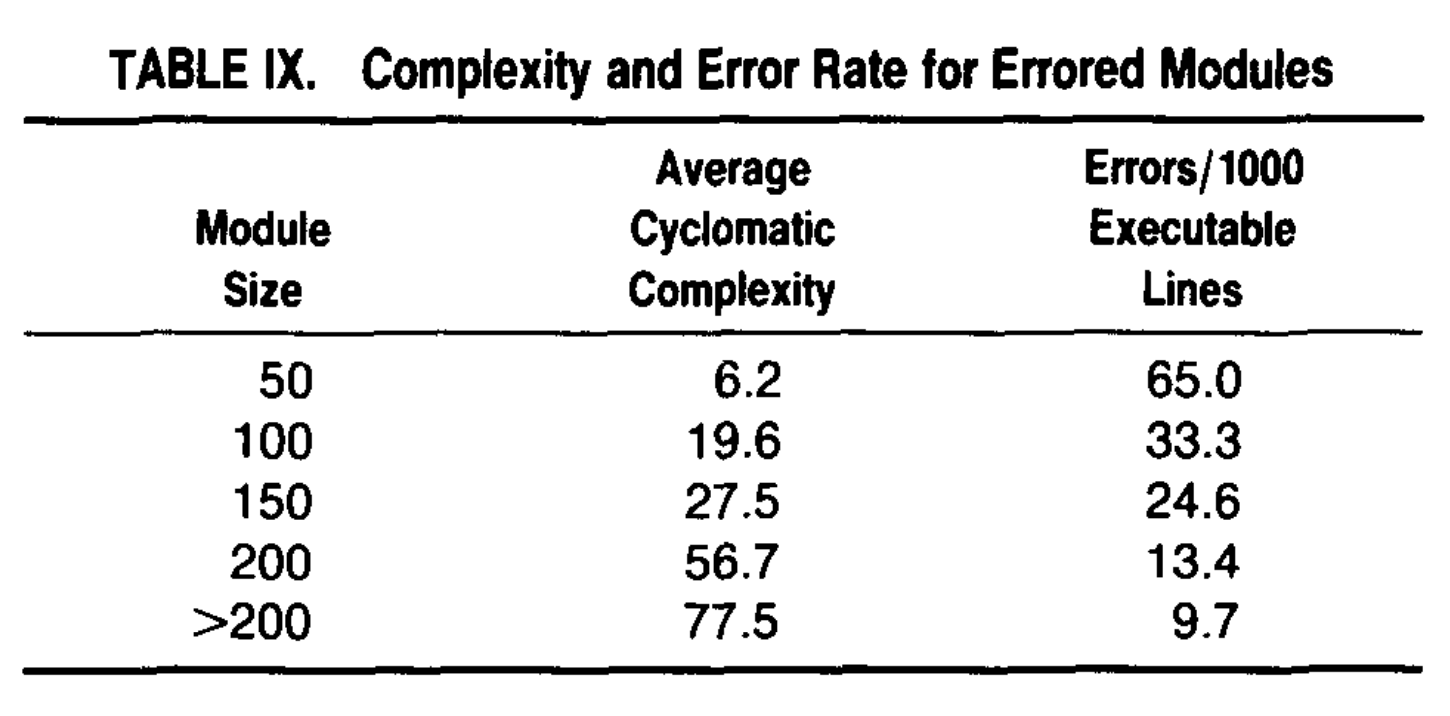
\includegraphics[width=\linewidth]{complexity.png}
\par\columnbreak\par
``One \ul{surprising} result was that module \ul{size} did not account for error proneness. In fact, it was quite the contrary---the larger the module, the \ul{less} error prone it was. This was true even though the larger modules were more complex.''\par
{\scriptsize Source: \bibentry{basili1984software}\par}
\end{multicols}}

\lnQuote
  {../18-defect-density/ieee-982}
  {A \ul{defect} is a product \ul{anomaly}. Examples include such things as 1)~omissions and imperfections found during early life cycle phases and 2)~faults contained in software sufficiently mature for test or operation.}
  {ieee982}

\lnPitch{\begin{multicols}{2}
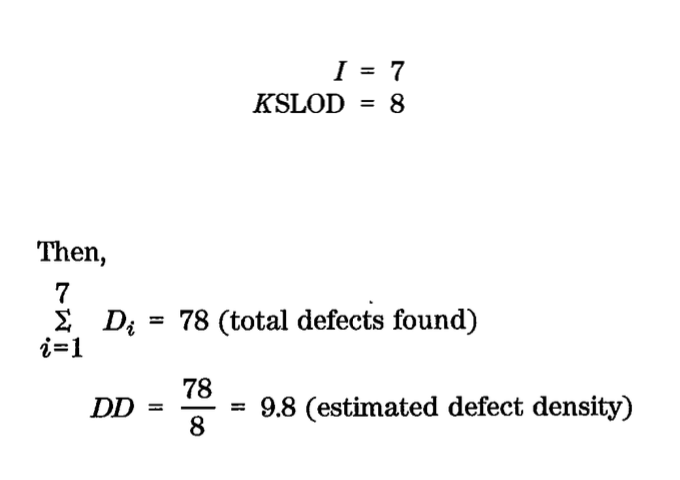
\includegraphics[width=\linewidth]{dd.png}
\par
{\scriptsize Source: \bibentry{ieee982}\par}
\par\columnbreak\par
``This measure has a degree of \ul{indeterminism}. For example, a low value may indicate either a good process and a good product or it may indicate a bad process. If the value is low compared to similar past projects, the inspection process should be examined. If the inspection process is found to be adequate, it should then be concluded that the development process has resulted in a \ul{relatively defect-free} product.''
\end{multicols}}

\lnPitch{
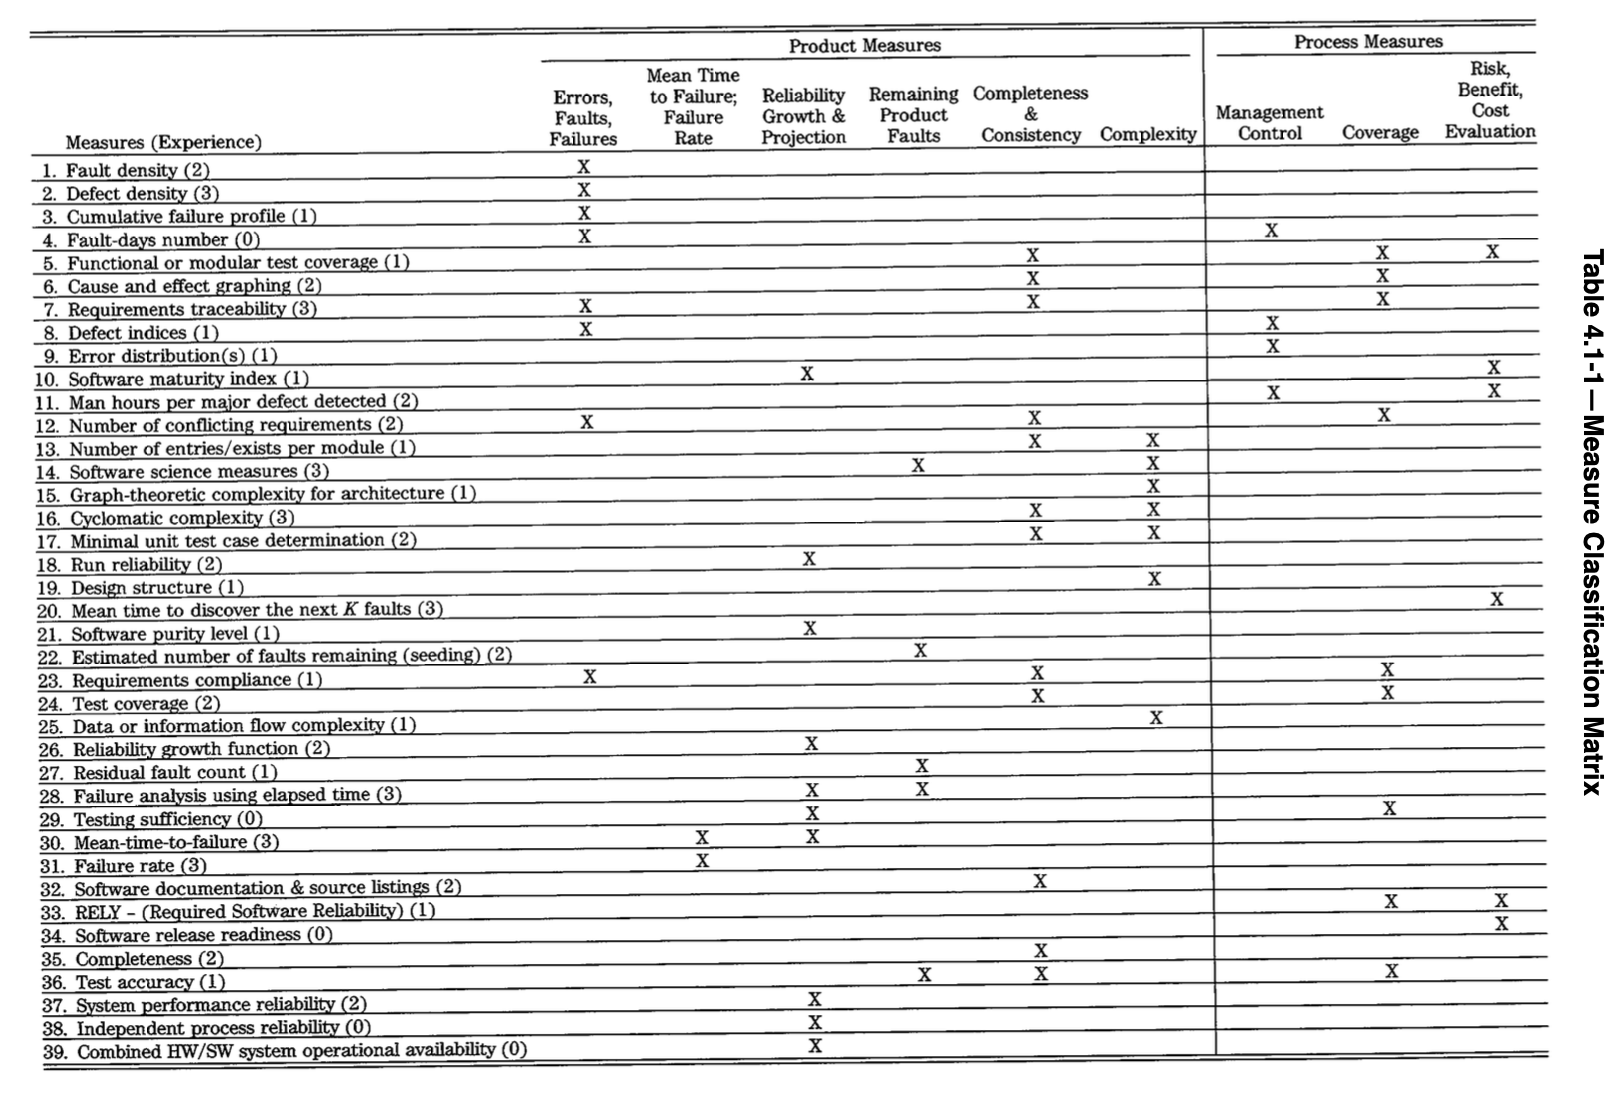
\includegraphics[width=.7\linewidth]{ieee-measures.png}
\par
{\scriptsize Source: \bibentry{ieee982}\par}}

\plush{\pptBanner{39 Measures for Reliable Software}
\begin{pptWide}{3}
\scriptsize\begin{enumerate}\setlength\itemsep{-.1em}
\item Fault Density
\item Defect Density
\item Cumulative Failure Profile
\item Fault-Days Number
\item Functional or Modular Test Coverage
\item Cause and Effect Graphing
\item Requirements Traceability
\item Defect Indices
\item Error Distribution(s)
\item Software Maturity Index
\item Manhours per Major Defect Detected
\item Number of Conflicting Requirements
\item Number of Entries and Exits per Module
\item Software Science Measures
\item Graph-Theoretic Complexity for Arch.
\item Cyclomatic Complexity
\item Minimal Unit Test Case Determination
\item Run Reliability
\item Design Structure
\item Mean Time to Discover the Next K Faults
\item Software Purity Level
\item Estimated Num. of Faults Remaining
\item Requirements Compliance
\item Test Coverage
\item Data or Information Flow Complexity
\item Reliability Growth Function
\item Residual Fault Count
\item Failure Analysis Using Elapsed Time
\item Testing Sufficiency
\item Mean Time to Failure
\item Failure Rate
\item Software Docmtn and Source Listings
\item RELY-Required Software Reliability
\item Software Release Readiness
\item Completeness
\item Test Accuracy
\item System Performance Reliability
\item Independent Process Reliability
\item Combined H\&S Operational Availability
\end{enumerate}
\end{pptWide}
\par
{\scriptsize Source: \bibentry{ieee982}\par}}

\lnQuote
  [Harlan D. Mills]
  {harlan-mills}
  {While our experience in applying statistical quality-control techniques to software development is limited, initial experience indicates that \ul{five fixes per thousand lines of code} can be tolerated without invalidating the application of statistics to estimate MTTF. This failure rate is low compared to normal development practices, where \ul{20 to 60} fixes per thousand lines of code is \ul{not atypical}.}
  {cobb1990engineering}

\lnQuote
  [Joseph Sherif]
  {joseph-sherif}
  {The analysis showed a \ul{significantly higher} density of defects during requirements inspections. It was also observed, that the defect densities found \ul{decreased} exponentialy as the mork products approached the coding phase.}
  {kelly1992analysis}

\lnQuote
  [Victor R. Basili]
  {victor-basili}
  {Five out of the six object-oriented metrics presented by \citet{chidamber1994metrics} appear to be useful to predict class fault-proneness during the high- and low-level design phases of the life-cycle.}
  {basili1996validation}

\lnQuote
  [Norman Fenton]
  {norman-fenton}
  {Our critical review of state-of-the-art of models for predicting software defects has shown that many methodological and theoretical \ul{mistakes} have been made... We recommend holistic models for software defect prediction, using Bayesian Belief Networks, as alternative approaches to the single-issue models used at present.}
  {fenton1999critique}

\lnPitch{\begin{multicols}{2}
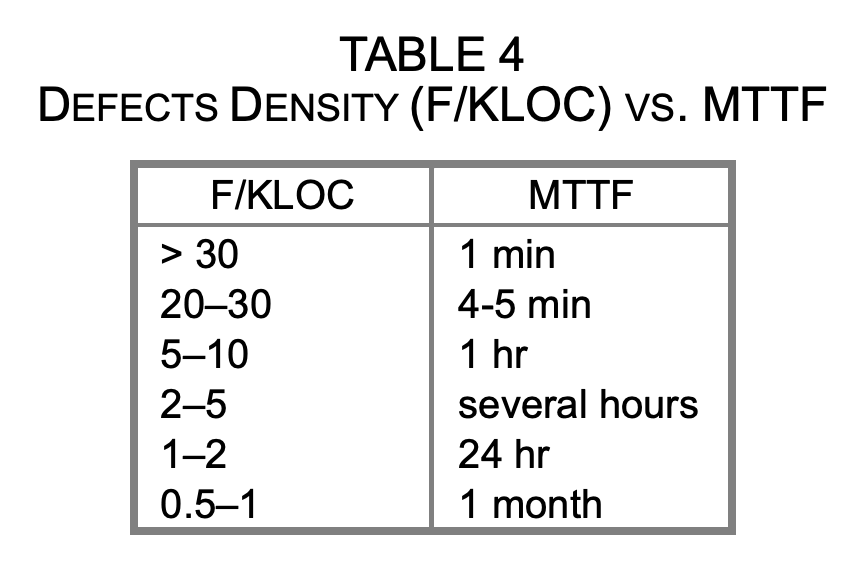
\includegraphics[width=\linewidth]{mttf.png}
\par\columnbreak\par
``This means we should be very wary of attempts to equate fault densities with failure rates, as proposed for example by~\citet{jones1996pragmatics}. Although highly attractive in principle, such a model does not stand up to \ul{empirical} validation.''\par
{\scriptsize Source: \bibentry{fenton1999critique}\par}
\end{multicols}}

\lnPitch{\begin{multicols}{2}
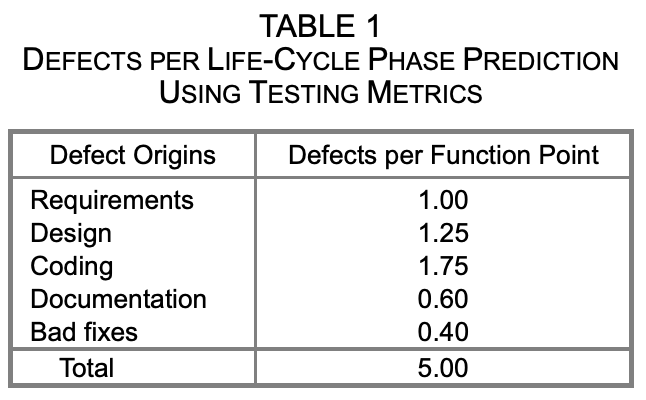
\includegraphics[width=\linewidth]{fps.png}
\par\columnbreak\par
``We already see defect density defined in terms of defects per \ul{function point}, and empirical studies are emerging that seem likely to be the basis for predictive models. For example, \citet{jones1991} reports the following bench-marking study, reportedly based on large amounts of data from different commercial sources.''\par
{\scriptsize Source: \bibentry{fenton1999critique}\par}
\end{multicols}}

\lnQuote
  [Steve McConnell]
  {steve-mcconnell}
  {Industry average experience is about 1-25 errors per 1000 lines of code for delivered software. Cases that have one-tenth as many errors as this are rare; cases that have 10 times more tend not to be reported. (They probably aren't ever completed!) Microsoft experiences about 10–20 defects per 1000 lines of code during in-house testing and 0.5 defects per 1000 lines of code in released product.}
  {mcconnell2004code}

\lnQuote
  [Parastoo Mohagheghi]
  {parastoo-mohagheghi}
  {The analysis showed that \ul{reused} components have lower defect-density than \ul{non-reused} ones. Reused components have more defects with highest severity than the total distribution, but less defects after delivery.}
  {mohagheghi2004empirical}

\lnQuote
  [Nachiappan Nagappan]
  {nachiappan-nagappan}
  {A case study performed on Windows Server 2003 indicates the validity of the relative \ul{code churn} measures as early indicators of system \ul{defect density}. Our code churn metric suite is able to discriminate between fault and not fault-prone binaries with an accuracy of 89\%.}
  {nagappan2005use}

\lnQuote
  [Thomas Ball]
  {thomas-ball}
  {Our results show that the \ul{static analysis} defect density is correlated at statistically significant levels to the \ul{pre-release} defect density determined by various testing activities. Further, the static analysis defect density can be used to predict the pre-release defect density with a high degree of sensitivity.}
  {nagappan2005static}

\lnQuote
  [A G{\"u}ne{\c{s}} Koru]
  {gunes-koru}
  {We studied four large-scale object-oriented products, Mozilla, Cn3d, JBoss, and Eclipse. We observed that defect proneness increased as class size increased, but at a \ul{slower} rate; smaller classes were proportionally more problematic than larger classes.}
  {koru2008investigation}

\lnQuote
  [Kazuhiro Yamashita]
  {kazuhiro-yamashita}
  {Although we found some support for findings in recent literature that \ul{smaller files} have higher defects density, we found further evidence that \ul{very large} or \ul{complex} files have lower defect densities and in some cases even lower defect proneness. Our findings have immediate practical implications: the redistribution of Java code into smaller and less complex files may be \ul{counterproductive}.}
  {yamashita2016thresholds}

\plush{\pptBanner{100+ Metrics that Predict Faults}
\begin{pptWide}{5}
\scriptsize\begin{enumerate}\setlength\itemsep{-.3em}
\item \textbf{\nospell{AHF}} Attribute Hiding Factor
\item \textbf{\nospell{AIF}} Attribute Inheritance Factor
\item \textbf{\nospell{COF}} Coupling Factor
\item \textbf{\nospell{MHF}} Method Hiding Factor
\item \textbf{\nospell{MIF}} Method Interface Factor
\item \textbf{\nospell{POF}} Polymorphism Factor
\item \textbf{\nospell{SCC}} Similarity-based Class Cohesion
\item \textbf{\nospell{ANA}} Average Number of Ancestors
\item \textbf{\nospell{CAM}} Cohesion Among Methods
\item \textbf{\nospell{CIS}} Class Interface Size
\item \textbf{\nospell{DAM}} Data Access Metric
\item \textbf{\nospell{DCC}} Direct Class Coupling
\item \textbf{\nospell{DSC}} Design size in classes
\item \textbf{\nospell{MFA}} Measure of Functional Abstraction
\item \textbf{\nospell{MOA}} Measure of Aggregation
\item \textbf{\nospell{NOH}} Number of hierarchies
\item \textbf{\nospell{NOM}} Number of Methods
\item \textbf{\nospell{NOP}} Number of polymorphic methods
\item \textbf{\nospell{LCC}} Loose class cohesion
\item \textbf{\nospell{TCC}} Tight class cohesion
\item \textbf{\nospell{ACAIC}}
\item \textbf{\nospell{ACMIC}}
\item \textbf{\nospell{AMMIC}}
\item \textbf{\nospell{Coh}} A variation on LCOM5
\item \textbf{\nospell{DCAEC}}
\item \textbf{\nospell{DCMEC}}
\item \textbf{\nospell{DMMEC}}
\item \textbf{\nospell{FCAEC}}
\item \textbf{\nospell{FCMEC}}
\item \textbf{\nospell{FMMEC}}
\item \textbf{\nospell{IFCAIC}}
\item \textbf{\nospell{IFCMIC}}
\item \textbf{\nospell{IFMMIC}}
\item \textbf{\nospell{OCAEC}}
\item \textbf{\nospell{OCAIC}}
\item \textbf{\nospell{OCMEC}}
\item \textbf{\nospell{OCMIC}}
\item \textbf{\nospell{OMMEC}}
\item \textbf{\nospell{OMMIC}}
\item \textbf{\nospell{ATTRIB}} Attributes
\item \textbf{\nospell{DELS}} Deletes
\item \textbf{\nospell{EVNT}} Events
\item \textbf{\nospell{READS}} Reads
\item \textbf{\nospell{RWD}} Read/write/deletes
\item \textbf{\nospell{STATES}} States
\item \textbf{\nospell{WRITES}} Writes
\item \textbf{\nospell{CBO}} Coupling between object classes
\item \textbf{\nospell{DIT}} Depth of inheritance tree
\item \textbf{\nospell{LCOM}} Lack of cohesion in methods
\item \textbf{\nospell{LCOM2}} Lack of cohesion in methods
\item \textbf{\nospell{NOC}} Number of children
\item \textbf{\nospell{NTM}} Number of trivial methods
\item \textbf{\nospell{RFC}} Response for a class
\item \textbf{\nospell{WMC}} Weighted methods per class
\item \textbf{\nospell{AMC}} Average method complexity
\item \textbf{\nospell{Past}} faults Number of past faults
\item \textbf{\nospell{Changes}} Number of times a module has been changed
\item \textbf{\nospell{Age}} Age of a module
\item \textbf{\nospell{Changeset}} Number of modules changed
\item \textbf{\nospell{\(N_1\)}} Total number of operators
\item \textbf{\nospell{\(N_2\)}} Total number of operands
\item \textbf{\nospell{\(g_1\)}} Number of unique operators
\item \textbf{\nospell{\(g_2\)}} Number of unique operands
\item \textbf{\nospell{AID}} Average inheritance depth of a class
\item \textbf{\nospell{LCOM1}} Lack of cohesion in methods
\item \textbf{\nospell{LCOM5}} Lack of cohesion in methods
\item \textbf{\nospell{Co}} Connectivity
\item \textbf{\nospell{LCOM3}} Lack of cohesion in methods
\item \textbf{\nospell{LCOM4}} Lack of cohesion in methods
\item \textbf{\nospell{ICH}} Information-flow-based cohesion
\item \textbf{\nospell{ICP}} Information-flow-based coupling
\item \textbf{\nospell{IH-ICP}} Information-flow-based inheritance coupling
\item \textbf{\nospell{NIH-ICP}} Information-flow-based non-inheritance coupling
\item \textbf{\nospell{CMC}} Class method complexity
\item \textbf{\nospell{CTA}} Coupling through abstract data type
\item \textbf{\nospell{CTM}} Coupling through message passing
\item \textbf{\nospell{NAC}} Number of ancestor
\item \textbf{\nospell{NDC}} Number of descendent
\item \textbf{\nospell{NLM}} Number of local methods
\item \textbf{\nospell{DAC}} Data abstraction coupling
\item \textbf{\nospell{DAC1}} Data abstraction coupling
\item \textbf{\nospell{MPC}} Message passing coupling
\item \textbf{\nospell{NCM}} Number of class methods
\item \textbf{\nospell{NIM}} Number of instance methods
\item \textbf{\nospell{NMA}} Number of methods added
\item \textbf{\nospell{NMI}} Number of methods inherited
\item \textbf{\nospell{NMO}} Number of methods overridden
\item \textbf{\nospell{NOA}} Number of attributes
\item \textbf{\nospell{NOAM}} Number of added methods
\item \textbf{\nospell{NOO}} Number of operations
\item \textbf{\nospell{NOOM}} Number of overridden methods
\item \textbf{\nospell{NOP}} Number of parents
\item \textbf{\nospell{NPAVG}} Average number of parameters per method
\item \textbf{\nospell{SIX}} Specialization index
\item \textbf{\nospell{C3}} Conceptual cohesion of Classes
\item \textbf{\nospell{McCabe}} Cyclomatic Complexity
\item \textbf{\nospell{Delta}} Code delta
\item \textbf{\nospell{Churn}} Code churn
\item \textbf{\nospell{Devs}} Number of developers
\item \textbf{\nospell{CLD}} Class-to-leaf depth
\item \textbf{\nospell{NOA}} Number of ancestors
\item \textbf{\nospell{NOD}} Number of descendants
\item \textbf{\nospell{LOC}} Lines of Code
\end{enumerate}
\end{pptWide}
\par
{\scriptsize Source: \bibentry{radjenovic2013software}\par}}

\lnQuote
  [Xiao Yu]
  {xiao-yu}
  {The problem of \ul{predicting} the precise number of defects via regression algorithms is \ul{far} from being solved.}
  {yu2022predicting}

\lnPitch{\begin{multicols}{2}
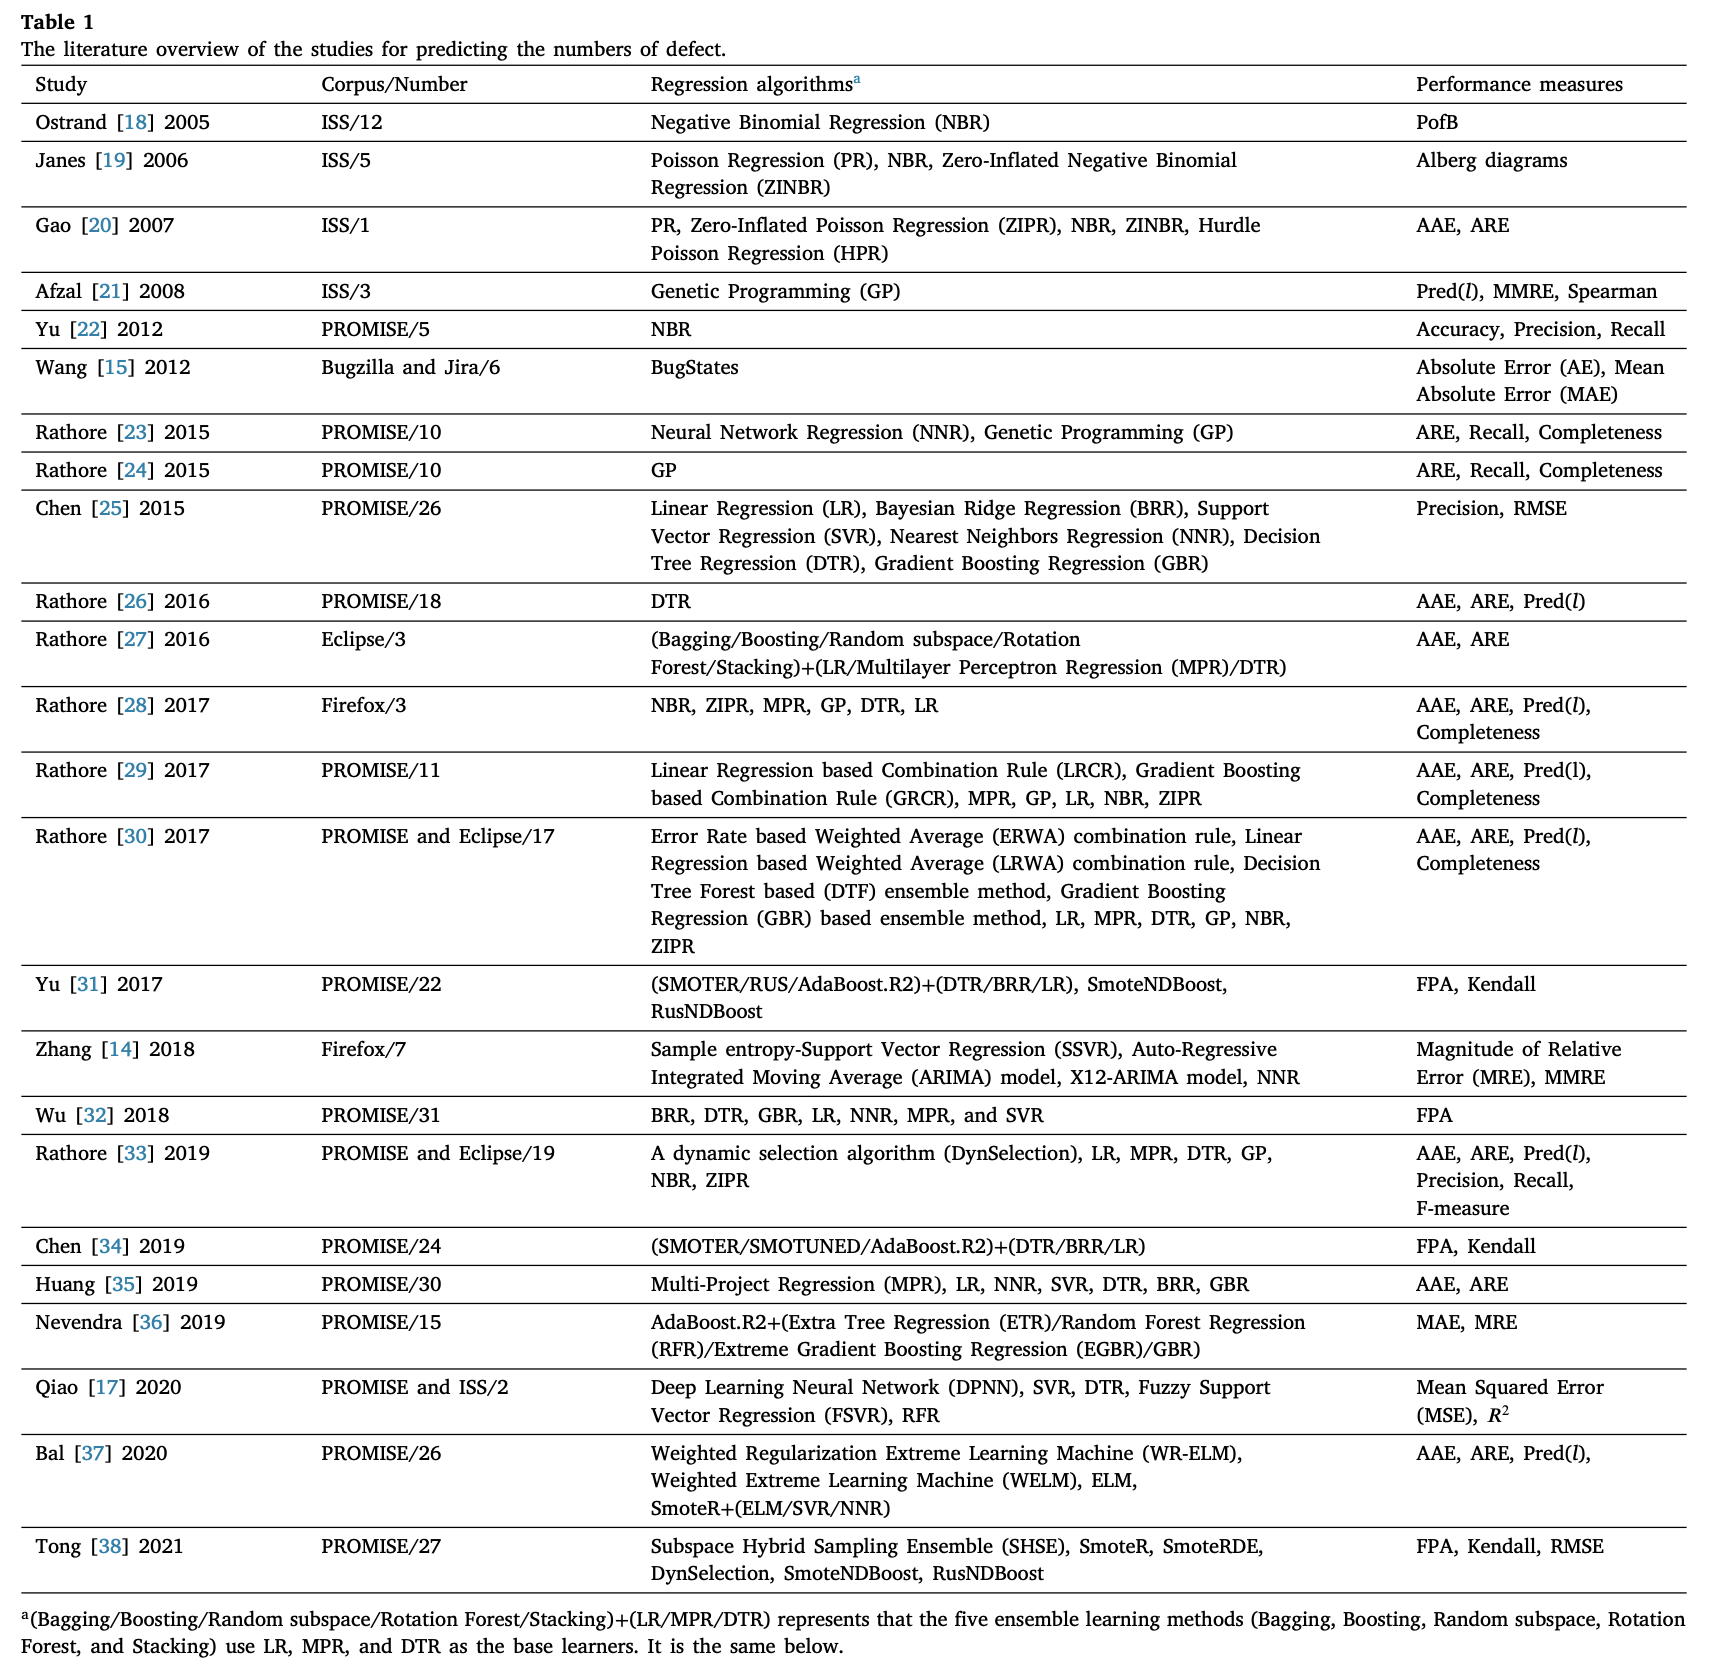
\includegraphics[width=.8\linewidth]{predicting-methods.png}
\par
{\scriptsize Source: \bibentry{yu2022predicting}\par}
\par\columnbreak\par
``Software testers want to not only know which software modules should be inspected first, but also evaluate the reliability and maintenance effort of each module. Therefore, they can first employ the historical data to construct a \ul{Defect Number Prediction} (DNP) model, then use the two trained models to predict the defective-proneness or the number of defects.''
\end{multicols}}

\lnPitch{\pptBanner{My Own Statistics (2 Feb 2024)}
{\ttfamily\small\begin{tabular}{llrrr}
\toprule
Github Repository & Stack & KLoC & Issues & I/KLoC \\
\midrule
\href{https://github.com/zerocracy/farm}{zerocracy/farm} & Java & 58 & 2343 & 40.4 \\
\href{https://github.com/objectionary/eo}{objectionary/eo} & Java & 49 & 2837 & 57.9 \\
\href{https://github.com/yegor256/cactoos}{yegor256/cactoos} & Java & 34 & 1707 & 50.2 \\
\href{https://github.com/yegor256/takes}{yegor256/takes} & Java & 27 & 1227 & 45.4 \\
\href{https://github.com/zold-io/zold}{zold-io/zold} & Ruby & 12 & 810 & 67.5 \\
\href{https://github.com/yegor256/tacit}{yegor256/tacit} & CSS & 1 & 227 & 227.0 \\
\bottomrule
\end{tabular}}\par
All repositories are open source.}

\end{document}
